\section{Reflections on our process}
In \autoref{sec:our-process} we described the process we used to organize our project workflow and how we incorporated parts of the scrum framework to better fit our project.
In this section, we reflect on our process and how it changed throughout the semester, as well as what we would change for our future projects.

\subsubsection{Scrum}
Our Scrum inspired process worked well with sprints, sprint planning, sprint backlog, product owner (PO), Scrum Master, planning poker, product backlog and product increment.
We took turns having the role as PO and Scrum Master.
The PO/Scrum Master had the task of planning the next product backlog and adding a DoD (definition of done) onto every task in the product backlog.
This person also had the responsibility of sending material to the supervisor, booking a conference room and conducting planning poker.
The sprint backlog and product backlog can be seen on \autoref{fig:trello-board}. 
This is a board on Trello we use to give an overview of how far people are with their tasks.
The leftmost column is the product backlog, the next four columns are the sprint backlog.
These are split into \textit{Sprint Backlog}, \textit{In progress}, \textit{In review} and \textit{Done}.

\begin{figure}[H]
    \centering
    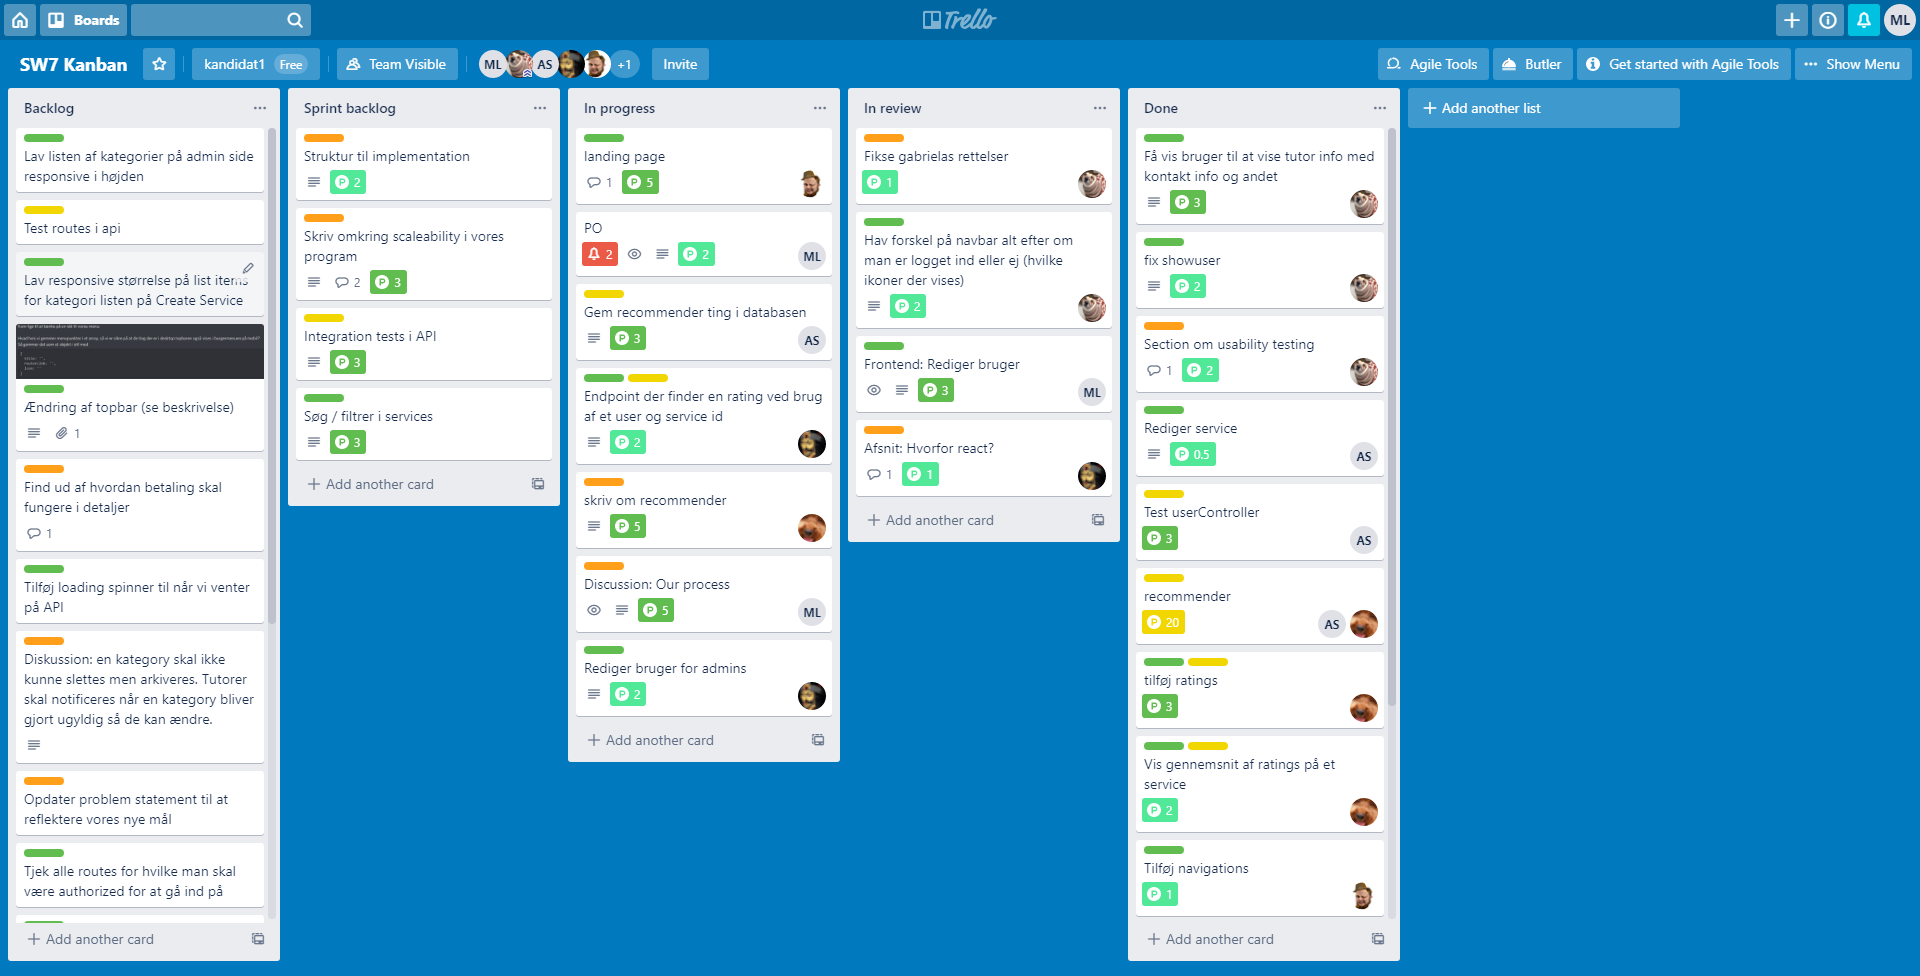
\includegraphics[width=0.8\linewidth]{figures/trellopicture.PNG}
    \caption{Our to-do board for the product and sprint backlog on Trello}
    \label{fig:trello-board}
\end{figure}
\noindent
When we conducted the sprint planning, we would use planning poker to estimate how many story points each task in the proposed sprint backlog should have.
The persons with the highest and lowest story points would discuss the reasoning behind their choice of points.
The story points were often very different if there were ambiguities, and people understood the tasks differently.
This gave everyone the same understanding of how the given tasks should be solved and eliminated most ambiguities. 
\\
However, as the project progressed and we started to develop the application and learning \textit{React}, the process started to become less systematic.
This was often due to it being difficult to estimate how long each task would take to solve.
When we were unable to estimate the tasks correctly, we would not finish them before the end of the sprint. 
This resulted in that our sprint backlog grew, as new tasks were assigned in a new sprint.
When we got more familiar with \textit{React} we were able to estimate how much the tasks would take, and the process got more systematic again.
\\\\
We also stopped conducting the retrospective meetings.
The Scrum Masters stopped enforcing the retrospective meetings so they started fading out.
These meetings could have helped make the project more structured as we could have discussed the problems that we faced and the reasons why we did not complete our tasks in time.

\subsubsection{Formal reviews}
The formal reviews were something that we changed in the middle of the semester, so that two people had to review a pull request together.
Previously, people would review a pull request individually.
Formal reviews were described in \autoref{sec:formal-reviews}.
The first part of every workday was spent on reviewing pull requests until all pull requests were reviewed.
\\\\
This increased the quality of the pull requests, as more errors were caught when two people had to debate the code.
This was especially important for big or difficult pull requests as it otherwise would be easier to just approve the pull request than to actually try and understand every part of it.
This is more time consuming and more difficult to plan, however.
If two people are in process of reviewing a pull request another person can be waiting for them to finish if they are assigned another pull request with one of them. 
When a pull request had been reviewed and changes were requested, the reviewers had to come back to review the changes made by the author.
To make this more organized we created a PR spreadsheet to give a better overview of which pull requests the developers were assigned to, and who was requested to do many or few reviews.
This can be seen on \autoref{fig:formal-reviews}.
\begin{figure}[H]
    \centering
    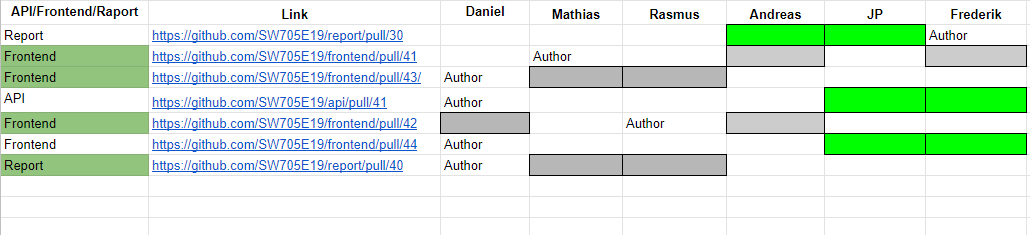
\includegraphics[width=\linewidth]{figures/formal-reviews.PNG}
    \caption{Pull request assignment sheet.}
    \label{fig:formal-reviews}
\end{figure}

\subsubsection{Prototypes}
In the beginning of the semester we created multiple prototypes for the entire system so that everyone had the same understanding of how the design should be.
Some of these prototypes have been described in \autoref{sec:prototypes-design}.
\\\\
When the development of the prototypes started we had two people assigned to the task of creating high fidelity prototypes, and afterwards people reviewed the prototypes and gave feedback and asked for changes.
Since the prototypes were high fidelity it was more difficult for reviewers to ask for big changes since it would take a lot of time to change.
There was an initial discussion of the design, but as they were developed it was harder for all developers to give input for the design.
A solution to this problem could be that the group developed low fidelity paper prototypes together. 
This would give the people assigned the task of creating high fidelity prototypes something to develop them from, and would also lessen the amount of changes they had to do from the feedback.
\\\\
When we started developing the application the prototypes were used a lot.
These were used for inspiration for every task, but later in the process they started to get used less often and lost a bit of their importance.
A reason for this could be that the developers were able to see the design pattern from other implemented pages, which could give them a good idea of how to solve the tasks.

\subsubsection{Working from home}
Unlike other semesters, we were not assigned a group room this semester.
This resulted in us working from home most days of the week, because we thought this would be easier and as productive as if we met at the university.
One of the cons of working from home is that it is more difficult to get help from the other group members, which can lead to people getting stuck on tasks.
After a few weeks we realized that it would be better if we had one workday together every week.
This was really beneficial as the more experienced React developers were able to help other members that were less experienced.
It was also easier to conduct sprint planning when we met in person.

\subsubsection{Supervisor meetings}
The day before the supervisor meeting we sent the report, a reading guide and an agenda for the meeting.
Our supervisor gave feedback on the material that we sent to her, and during the meeting we presented the things that we had done the previous week.
These meetings have been longer than the meetings we had previously experienced in previous semesters, but this also resulted in better feedback, as the questions she asked made us reflect on certain choices we had made.

\subsubsection{What we would do differently}
One of the problems that we faced was that people could get stuck on tasks.
For future projects we will try to be more aware of where people are in the process, so that it would be easier to help them with solving their tasks.
One of the solutions to this could be daily standups, so that we are aware of where people are with their tasks, and which ones they have not completed.
Another solution could be to have more workdays at the university, so that people have an easier time getting help from one another.
It is especially important in the beginning of the semester when there are still a lot of ambiguities and uncertainties with the project.  
We would also like to hold the retrospective meeting so that we had to reflect on the previous week and correct the problems that we faced.
When adding tasks to the product backlog it should also be a requirement to add a DoD, since we experienced being unable to recognize what needed to be done from just the title.
